\chapter{Negation}

\epigraph{We would not say, ``I don't have it.''
Instead, we say, ``It hasn't yet come to me.'' That difference
is everything.}{}

\is{negation|(}Negation is a topic that seems extremely simple on the surface, but its underlying complexity makes it a great vehicle for understanding so many areas of the language landscape: \is{scope|(}scope, \is{polarity (positive vs negative)|(}polarity, \is{language change|(}language change, \is{grammaticalization|(}grammaticalization, and \is{exaptation}exaptation.

\section{Language change, grammaticalization, and exaptation}

``I heard not of it before,'' says Bertram in Shakespeare's \textit{All's well that ends well}. You and I would say \textit{I have not heard of it before}.

Language~-- as you can clearly see~-- changes. But the changes are often surprisingly systematic.

\il{English!Old|(}Old English (450--1150 CE) used \textit{ne}, simply placed before the verb, for negation. Take (\ref{ex:ne-habbe}) for example.

\ea \label{ex:ne-habbe}
    \gll \textit{Ne} \textit{hæbbe} \textit{ic} \textit{hit} \textit{ær} \textit{gehīered} \\ no(t) have I it before {heard of} \\
    \trans `I have not heard of it before.'
\z

If things had stayed this way,\footnote{Actually, there is a construction in which things more or less have: \textit{Never have I \dots}} then the language-learner strategy of putting \textit{no} before the relevant verb (\textit{I no put it there}) would be basically the right one. It's simple, and many of the world's languages do essentially this.

But this is just one stage in what's known as \is{Jespersen's cycle|(}Jespersen's cycle.\footnote{I derive most of the following stylized description from Chapter 1 of \ia{Jespersen, Otto}\citet{Jespersen1917}.} Here's how it goes (see Figure~\ref{fig:Jesp-cycle}).

\subsection{Jespersen's cycle}

\paragraph*{Stage one}
There's a problem with \textit{no} (or \textit{ne}, or \textit{non}, etc.) hanging out there on its own before the verb: that initial negator often gets swallowed up when your speech apparatus fails to engage quite in time. Think about saying \textit{Good morning!} That \textit{good} is often hardly voiced at all: \textit{G'morning!}. Do people reliably say \textit{I'm afraid not} with the subject \textit{I}, \textit{am}, and first syllable of the next word? \textit{'fraid not}. \textit{See you later} is missing \textit{I} and \textit{will} in their entirety, and \textit{'kay} is short for \textit{OK}, itself a slangy shortening of \textit{oll korrect} (`all correct'), from a brief Bostonian fad of humorous initialisms in the early 1800s \citep{OK}. The start of a phrase is a perilous place for words to find themselves if they want to stick around.

Phrase-initial \textit{ne} was at risk of erosion. And in due course, the stressed version in Old English gave way to unstressed, which, in turn, simply gave way. But not quite yet.

\paragraph*{Stage two}

The gradual erosion of phrase-initial elements creates little problem for cases like \textit{Morning!} or \textit{Afraid not.} But phrase initial \textit{ne} carries a meaning fundamentally different from the same sentence without it. Without a clear, reliable marker of negation, the negative meaning is often lost entirely.

To compensate for a degraded \textit{ne}, even before it had edged its way out of English entirely, we began adding extra elements to ensure the negative meaning wasn't missed. For example, the Old English \textit{nā} in (\ref{ex:ne-sceal}) directly negated nouns or adjectives, as in \textit{nā good} meaning `no(t) good'. And it was used together with \textit{ne}.

\ea \label{ex:ne-sceal}
    \gll \uline{\textit{Ne}} \textit{sceal} \uline{\textit{nā}} \textit{man} \textit{mid} \textit{worde} \uline{\textit{nē}} \textit{mid} \textit{dǣde} \uline{\textit{nān}} \textit{yfel} \textit{dōn}  \\ no(t) schall no man with word nor with deed no evil do \\
    \trans `No man shall do any evil, neither in words nor in deeds.'
\z

Today, \textit{\uline{no} man shall \uline{not} do any evil} would mean that every man will do some evil. In Old English, though, that particular phrasing was emphatically negative. Of course, the same strategy in \textit{I \uline{don't} do \uline{no} evil} is perfectly clear to \is{Standard English}Standard English speakers today, and anybody claiming those two negatives make a positive is, in fact, doing evil with words. The contemporary \textit{\uline{No} man shall do any evil, \uline{neither} in words \uline{nor} in deeds} has three negatives, each propping up the next. So-called ``\is{negation!double negation}double negatives'' are still with us in some form, even in Standard English.

This is the birth of today's \textit{not}, which comes from \textit{noht} (from \textit{nought}/\textit{nowiht}, meaning `nothing').  \textit{Ic ne secge} `I no say' was strengthened by adding this word, as in \textit{ic ne secge nowiht} `I no say nothing.' But this  strategy to reinforce the meaning made the word \textit{ne} even more vulnerable to disappearance, and disappear it did. 

\paragraph*{Stage three}

The decline and eventual disappearance of \textit{ne} continued through \il{English!Middle}Middle English (1150--1500~CE), making way for the rise of \textit{not}. Consider the phrase \textit{I ne knowe not} `I no know not(hing)', a linguistic crossroads of sorts. In a process called \textsc{grammaticalization}, \textit{not} was being bleached of its `nothing' meaning and becoming simply a marker of negation, equivalent to \textit{ne}. For a time, it could be understood as either `I know nothing' or simply as `I know not', but eventually, new generations of speakers forgot the `nothing' meaning or never learned it in the first place.

Late in stage 2, this new \textit{not} was even obligatorily paired with \textit{ne}, as in the \il{French}French \textit{Je \uline{ne} sais \uline{pas}}, propelled by the evolving sound patterns of English, coupled with the desire for clear and unambiguous communication.

As Old English\il{English!Old} segued into Early Modern English\il{English!Early Modern} (1500--1700 CE), with the devoicing of \textit{ne} and the redundancy of two negators on opposite sides of the verb, \textit{ne} completed its disappearing act, and double negatives lost favour. The early grammarians of Late Modern English (1700--Present) seem to have thought them obsolete by 1762 \citep[365]{Gilman1989}.

But that's only half the story.

\paragraph*{Stage four}

\textit{Not} arrived late in English and it was positioned late in the sentence, which caused a bit of a problem. In \il{German}German, where a similar process occurred, the negator \textit{nicht} can be delayed a lot, isolating it from the much earlier verb location,

\begin{quote}
    the result being that the hearer or reader is sometimes bewildered at first and thinks that the sentence is to be understood in a positive sense, till suddenly he comes upon the \textit{nicht}, which changes everything. \\ \citep[10]{Jespersen1917}
\end{quote}

English was saved from this kind of confusion by another change that was going on around the same time, a proliferation of uses of \textit{do}.\footnote{For a less stylized account of \textit{do}, see \citet{Denison1985}.}

One thing that \textit{do} did was to add emphasis: \textit{do come and see us, darling} may not have been any more sincere then than it is now, but at least it \strong{sounds} emphatic. It was also stressed. And there were already other auxiliary verbs which were followed by \textit{not}: \textit{I could not go}, \textit{it might not rain}, etc. This emphatic \textit{do}, with its exaggerated stress, was a perfect candidate for hosting the negator. The end result was \is{do-support@\textit{do}-support|(}\hyperref[sec:sec:basic-do-support]{\textit{do} support}, where the auxiliary \textit{do} serves as a solid anchor for \textit{not}, preventing any ambiguity about the presence of negation.\is{auxiliary do@auxiliary \textit{do}|(}

\textit{Do} started out as a mere helper but quickly became an indispensable part of English negation. By the time of Early Modern English, constructions without \textit{do}, like \textit{I know not}, became increasingly rare and marked as formal or archaic. The rise of \textit{do} in negation coincided with its spread in other constructions as well, such as \is{interrogative clause|(}interrogatives (\textit{Do you know?}) and emphatics (\textit{I do want that}). \textit{Do}-support is unique to English among the Germanic languages.

\paragraph*{Stage five}

With the establishment of \textit{do} as a crucial part of negation, \textit{not} once more became dispensable, or at least reducible. A new variation emerged: \is{contraction|(}contraction with \textit{do not} naturally evolving into \textit{don't}. Other forms followed suit: \textit{does not} \rightarrow ~\textit{doesn't}, \textit{did not} \rightarrow ~\textit{didn't}. And contracted forms of other auxiliary verbs cropped up: \textit{can't}, \textit{won't}, \textit{isn't}, even \textit{amn't} for a while.

These contractions (now \is{negative!inflection in modal auxiliaries}negative inflections) have become so ingrained in the language that the uncontracted forms can sound overly formal, even pedantic, in everyday conversation.

\begin{tcolorbox}[title=\is{auxiliary verb!negative form}Negative auxiliary verbs, colback=white]\is{contraction}

You may have been told to write \textit{do not} instead of \textit{don't}, \textit{is not} instead of \textit{isn't}, \textit{will not} instead of \textit{won't}, etc. If so, you were misguided. 

\phantom{fri}Prior to the 1600s, \textit{not} was obligatorily stressed, but in the early 1600s, it started to lose that requirement. In writing, the new unstressed form was sometimes spelled \textit{--n't}, especially in comedic plays and when characters with country accents or nonstandard dialects spoke \citep{Brainerd1989}. This is the origin of the stigma and the subsequent avoidance.

\phantom{fri}Fast forward to the 19th and 20th centuries and you'll find \textit{--n't} popping up everywhere in writing~-- not just in plays and novels, but also in personal letters, newspapers, and various descriptions. In the 21st century, \textit{--n't} is ubiquitous. Proscribing its use in formal writing is a pedantic and outdated view. In reality, these forms are not only efficient but also reflect the natural rhythm of today's language. Their use should be embraced, not shunned

\end{tcolorbox}

\paragraph*{Stages six and seven}

\begin{figure}
    \centering
\begin{tikzpicture}[
  node distance=1cm,
  arrow/.style={-{Triangle[length=3mm, width=2mm]}, line width=1mm},
  faded/.style={arrow, red!40},
  dropped/.style={arrow, gray},
  solid/.style={arrow, black},
  align=center
]



  % Nodes
  \node (i1) {1.~~~Ic};
  \node[right=10pt of i1] (ne1) {ˈne\phantom{I}};
  \node[right=10pt of ne1] (know1) {wat\phantom{I}};
  \node[right=10pt of know1] (donot1) {\phantom{do notI}};
  
  \node[below=of i1] (i2) {2.~~~I};
  \node[below=of ne1] (ne2) {ne\phantom{I}};
  \node[below=of know1] (know2) {know\phantom{I}};
  \node[below=of donot1] (not2) {noht\phantom{I}};
  
  \node[below=of i2] (i3) {3.~~~I};
  \node[below=of ne2] (ne3) {\phantom{netI}};
  \node[below=of know2] (know3) {know\phantom{I}};
  \node[below=of not2] (not3) {not\phantom{I}};
  
  \node[below=of i3] (i4) {4.~~~I};
  \node[below=of ne3] (do4) {\phantom{neI}};
  \node[below=of know3] (not4) {do\phantom{I}};
  \node[below=of not3] (know4) {not\phantom{I}};
  \node[right=10pt of know4] (new4) {know\phantom{I}};
  \node[right=10pt of new4] (any4) {\phantom{anythingI}};

  
  \node[below=of i4] (i5) {5.~~~I};
  \node[below=of do4] (do5) {\phantom{neI}};
  \node[below=of not4] (not5) {don't\phantom{I}};
  \node[below=of know4] (know5) {\phantom{notI}};
  \node[below=of new4] (new5) {know\phantom{I}};

  
  \node[below=of i5] (i6) {6.~~~I};
  \node[below=of do5] (do6) {\phantom{neI}};
  \node[below=of not5] (not6) {dunno\phantom{I}};
  \node[below=of know5] (know6) {anythin'\phantom{I}};
  \node[below=of new5] (new6) {\phantom{knowI}};
  \node[right=10pt of new5] (any6) {anything\phantom{I}};

  \node[below=of i6] (i7) {7.~~~I};
  \node[below=of do6] (do7) {\phantom{neI}};
  \node[below=of not6] (not7) {know\phantom{I}};
  \node[below=of know6] (know7) {\uline{\textit{en}}\phantom{t}};
  \node[below=of new6] (new7) {\phantom{knowI}};

  
  % Arrows
  \draw[solid] (ne1) -- (ne2);
  \draw[dropped] (ne2) -- (ne3);
  %\draw[faded] (ne3.center) -- (do4);
  \draw[solid] (know1) -- (know2);
  \draw[solid] (know2) -- (know3);
  \draw[solid] (know3) -- (new4);
  \draw[faded] (donot1) -- (not2);
  \draw[solid] (not2) -- (not3);
  \draw[solid] (not3) -- (know4);
  \draw[faded] (ne3) -- (not4);
  \draw[solid] (not4) -- (not5);
  \draw[solid] (know4) -- (not5);
  \draw[solid] (new4) -- (new5);
  \draw[solid] (new5) -- (not6);
  \draw[solid] (not5) -- (not6);
  \draw[solid] (any6) -- (know6);
  \draw[solid] (know6) -- (know7);
  \draw[solid] (not6) -- (not7);
  \draw[faded] (any4) -- (any6);

\end{tikzpicture}
    \caption{Stylized illustration of Jespersen's cycle from Old English to a possible future English.}
    \label{fig:Jesp-cycle}
\end{figure}

And still the contractions keep contracting. The /t/ on the end of \textit{can't} is hardly audible most of the time, and the only way to distinguish between it and its positive form is the difference in their vowels (/kən/ vs /kæn/). \textit{Don't} with \textit{wanna} is a truncated /doʊ/, and, together with \textit{know}, we get \textit{I dunno}, the negator and verb fused into a single word, \textit{don't} little more than a prepended \textit{d} sound.\footnote{In fact, you can just sort of intone the standard pitches of \textit{I don't know} without so much as moving your lips and you'll usually be understood.}

This brings up the possibility that we've cycled back to stage 2, where we're reaching for another element to shore up the negative. It could be anything, but perhaps, this time it \strong{will} be \textit{anything}. It's possible to imagine a future English in which \textit{don't} is diminished to the point where people start using \textit{anything} obligatorily, where it starts to have its central meaning bleached away, and where it becomes the new negator.

The stressed syllable in \textit{anything} is /ˈɛ/, so perhaps, this new `not' is reduced to \textit{en}. Is it likely? I think en, but we'll have to wait and see.


%Since Old English, \textit{do} had had a causative meaning, so that \textit{did down fell} could mean `felled' or `caused to be felled'. But \textit{fell} itself has a causative meaning: if you fell a try, you cause it to fall down by cutting it. And so \textit{did} can be understood as having no real meaning but simply marking the past tense (semantic bleaching leading to grammaticalization). 

%\ea \label{ex:did-doun-felle}
%    \gll \textit{Henry...} \textit{þe} \textit{walles} \textit{did} \textit{doun} \textit{felle}, \textit{þe} \textit{tours} \textit{bette} \textit{he} \textit{doun}. \\ Henry the walls did down fell, the towers beat he down \\ \trans `Henry made the walls fall, the towers he beat down.'
%\z

%Employing \textit{do} like this was particularly useful in poetry. Here, it allows \textit{walles} to rhyme with \textit{felle} (both of which have two syllables), and it adds padding to preserve the meter of the line. It was handy, giving the poet had the option to use \textit{do} + \textsf{verb} or just \textsf{verb}, depending on rhyming and metrical needs. \footnote{Indeed, we see the same thing in Modern English poetry, as in \textit{The ice did split with a thunder-fit; The helmsman steered us through!} from The Rime of the Ancient Mariner by Samuel Taylor Coleridge.}

%But this poetic ``periphrastic \textit{do}''~-- so called because it's a paraphrase of the simple verb~-- sparks a fashion for periphrastic \textit{do} in prose and general use.



%Initially, negation in English did not require an auxiliary verb. Sentences like \textit{I know not} or \textit{He comes not} were standard. However, as the language evolved, the auxiliary \textit{do} began to appear in negative constructions, a phenomenon not observed in most other Germanic languages.

%\textit{Do-support} became especially prominent in the \textit{Early Modern English} period. The syntax of negation shifted from simply placing \textit{not} after the main verb, to using \textit{do} as a necessary component in forming negatives. For example, \textit{I know not} transitioned into \textit{I do not know}, and \textit{He comes not} became \textit{He does not come}.

%This shift can be attributed to several factors. One theory suggests that the rise of \textit{do-support} was a means to disambiguate sentences where the initial negation particle, like \textit{ne}, was being phonetically reduced and less discernible. By introducing \textit{do}, the negation was made clearer and more emphatic.

%Another perspective links this change to the broader simplification of verb forms in English. As the language shed much of its inflectional morphology, the auxiliary \textit{do} provided a way to maintain syntactic distinctions that were previously marked by verb endings.

%\textit{Do-support} in negation also aligns with the general trend of English becoming more analytic, moving away from a reliance on inflectional forms to express grammatical relationships. The auxiliary \textit{do} in negative constructions exemplifies this analytical tendency, marking a significant departure from the synthetic structures of Old and Middle English.

%By the time of Shakespeare and beyond, \textit{do-support} in negation had become firmly established in English. This syntactic innovation was not merely a grammatical quirk but reflected deeper changes in the language's structure and its speakers' communicative needs.

\paragraph*{Summary}

We all know that language changes. Some of us may have the pre-modern idea that we speak a fallen language, an idea rooted in the concept of a golden age or a primordial state of grace from which English has since degenerated, though no one is really sure what that was or when it presided. I hope this stylized history and weak attempt at prognostication suggest to you that language change too is rule governed, natural, and eternal, not simply the accumulated rust of a once gleaming metal exposed to the elements. It is decidedly not the case that one can simply look at the way English is today and discern some kind of logical structure, but the structure is there, and the logic behind it can be uncovered.

I've seen many teachers say that English is crazy or illogical. It isn't. Like any language, it's a wonderful, complex, massively-multi-player game with many interacting logics. Moreover, suggesting that English is crazy or arbitrary to folks who are learning it~-- whether learning to speak it or learning to teach it~-- is counterproductive. Telling learners that English is illogical can foster unnecessary apprehension or even disillusionment. Students don't have to know the history of every word and grammatical system, but, for teachers, understanding something about the structure of language change and the forces driving it reveals that there are reasons and explanations if we're interested in looking for them. It helps us to approach teaching and learning with a sense of curiosity and discovery, rather than frustration and confusion.

The most important idea behind this potted history and projected future of negation is that forms come and go for reasons. Many of the errors that English-language learners make stem from those same reasons, and the mistakes often recapitulate plausible past or future forms of the language; they follow the logic that drives language change. Recall how \textit{pease} became \textit{peas} (Section \ref{sec:count})? It was a mistake, but it made so much sense to so many that it overwhelmed the original form. Likewise, students' mistakes are often insightful and motivated, not foolish or risible.

This is not an attempt to justify an anything-goes attitude. \href{ch:standards}{Standard English} is real, and students of English will mostly want to learn the Standard variety. Patterns like \textit{I no go} should be recognized as the mistakes they are, but they should not be cause for frustration or distress on your part or your students'. And again, I ask you to recall that when language learners make the correct choice, you should respect them for their insight into the peculiar way of looking at the world shared by English speakers. For your part, understanding how the language works often provides insight into where the confusion is coming from. It allow teachers to point out analogous aspects that are already familiar or that may be next points of departure, and to suggest ways to improve.
\is{Jespersen's cycle|)}
\is{language change|)}


\section{Scope}
The scope of a problem is how big it is, how many things it impacts. A small-scope project might involve developing a single mobile application for a local business, while a large-scope project could be constructing a multi-functional smart city infrastructure. The scope of an investigation is the breadth and diversity of the questions asked, while a law's scope refers to the range of activities, individuals, or situations it covers. In $5\times3+2$, the multiplication operator has scope only over $5$ and $3$, while in $5 \times (3 + 2)$, it has scope over $5$ and $3+2$. In the realm of programming, the scope of a variable dictates where the variable can be accessed or modified within the code.

\textsc{Scope} is like that in linguistics too. If one element has scope over some part of a clause or phrase, then it has a semantic effect on that part. Take the negative sentence \textit{I didn't finish my homework because I was at the park}. What is within the scope of negation? In the most obvious reading, the homework was not completed, and the reason for my failure to do so was that I was at the park. Here the scope of negation includes only \textit{finish my homework}. That's what didn't happen. But there is a second reading in which everything after \textit{didn't} is in the scope of negation. Under this reading, I'm negating the whole claim that I finished my homework \strong{because I was at the park}. In other words, it was not being at the park that resulted in my homework getting finished.

Or consider (\ref{ex:not-many}). In (a) \textit{many} is within the scope of negation: the number of friends who came is small. In (b) \textit{many} is outside the scope of negation: the number of friends who did not come is large.

\ea \label{ex:not-many}
    \ea[]{\textit{Not many friends came.}}
    \ex[]{\textit{Many friends didn't come.}}
    \z
\z

\noindent These may seem like the same thing, but if you have only a few friends, then (a) could be true while (b) would be false, a semantic difference.

%Scope is not limited to negation. Quantifiers like \textit{all}, \textit{some}, and \textit{none} also have scope implications. In the sentence \textit{All students read some books}, the scope of \textit{all} and \textit{some} determines whether the sentence means each student reads some (possibly different) books, or there are specific books that all students read. This ambiguity arises from the different possible scopes of the quantifiers.

\subsection{Scope and modal auxiliary verbs}

Interestingly, \is{modal auxiliary verb|(}modal auxiliary verbs have different implications for scope of negation. Consider (\ref{ex:can-vs-must}).

\begin{multicols}{2}
\ea \label{ex:can-vs-must}
    \ea \label{ex:can}
        \ea[]{\textit{You can do it.}}{`you're able to'}
        \ex[]{\textit{You can't do it.}}{`you're \uline{un}able to'}
    \z
    \ex \label{ex:must}
        \ea[]{\textit{You must do it.}}{`you're obliged to'}
        \ex[]{\textit{You mustn't do it.}}{`you're obliged to \uline{not}'}
        \z
    \z
\z
\end{multicols}

If you can do something, you're able to do it. There are two ways to negate this: 1) you are unable to do it, and 2) you're able not to do it, to avoid doing it. The only way to read \textit{can't} in (\ref{ex:can}) is the first way, with ability negated. So here we say that negation has scope over the modal; \textit{can do it} is negated.

In the rare case that you want to use \textit{can} to say you're able to avoid doing it, then the normal way is to say \textit{you can not do it} (e.g., \textit{It's OK, you can not go to school today.}), with a deliberate pause before \textit{not}. 

When we go through the same analysis with \textit{must}, we get a different result. If you must do something, you're obliged to do it. There are again two ways to negate this: 1) you are not obliged to do it, a lack of obligation, and 2) you're obliged not to do it, a prohibition. The only way to read \textit{mustn't} in (\ref{ex:must}) is the second way, as a prohibition. So here we say that negation does not have scope over the modal; only \textit{do it} is negated, not \textit{must}.

Here, there is no simple way to negate \textit{must} without resorting to completely different constructions or vocabulary, such as \textit{it is not the case that you must do that} or more simply \textit{you're not obliged to}.

\textit{Mustn't} (or \textit{must not}) and  is unusual here. Most of the negative modal auxiliary verbs are like \textit{can't}, which is to say their modal meaning falls within the scope of negation.
\is{modal auxiliary verb|)}

\section{Types of negation} \label{sec:types-of-negation}

There is an appealing, but ultimately incorrect sense that scope of negation is related to types of negation: clausal (including verbal \& non-verbal) negation, sub-clausal negation, and affixal negation. But it is not the case that clausal negation has scope over the whole clause or that affixal negation has scope only over a word.\footnote{See Chapter \ref{ch:vocabulary} for more on affixation and morphology.} Nevertheless, it's useful to understand the different types of negation because of how it affects other parts of the sentence.

The seeming relationship is due to the intuition that, if a negative marker lacks scope over a verb, the verb, and therefore the clause, is not negative. And yet we've already seen that \textit{can't} and \textit{mustn't} scope differently. I assure you that both of the (i) examples in (\ref{ex:can-vs-must}) are examples of verbal negation, which means they're examples of clausal negation even though their scope is quite different.

How can this be? Once again, it's because of the difference between \is{syntax vs semantics}syntax and semantics. Scope is a semantic concept, while the different types of negation are syntactic types. Semantically, \textit{can't} and \textit{mustn't} are different. Syntactically, they're the same.

To the types of negation listed above (clausal, including verbal \& non-verbal, sub-clausal, and affixal), we can add various constructions that result in pragmatic negation. See Figure~\ref{fig:neg-types}.

\begin{figure}
    \centering
    \begin{tikzpicture}[
      node distance=2cm,
      mynode/.style={
        ellipse,
        draw,
        align=center
      },
      myarrow/.style={
        -Stealth
      }
    ]

    % Nodes
    \node[mynode] (neg) {Negation};
    \node[mynode, below left=of neg] (clausal) {Clausal};
    \node[mynode, below=of neg] (subclausal) {Sub-Clausal};
    \node[mynode, right=of subclausal] (affixal) {Affixal};
    \node[mynode, below=of clausal] (verbal) {Verbal};
    \node[mynode] (nonverbal) at ($(subclausal.south)!0.5!(verbal.east) + (1cm, -1cm)$) {Non-Verbal};

    % Adjusted implicit node positioning and dimension with rotated text
    \node[mynode, minimum height=3cm, minimum width=0.8cm, text width=0.8cm, right=of clausal, yshift=-2cm, xshift=1cm] (implicit) {\rotatebox{270}{Pragmatic}};

    % Lines
    \draw[myarrow] (neg) -- (clausal);
    \draw[myarrow] (neg) -- (subclausal);
    \draw[myarrow] (neg) -- (affixal);
    \draw[myarrow] (clausal) -- (verbal);
    \draw[myarrow] (clausal) -- (nonverbal);

    \end{tikzpicture}
    \caption{Types of negation}
    \label{fig:neg-types}
\end{figure}




\subsection{Clausal negation} \label{sec:clausal-negation}
\nopagebreak[4]
\is{negation!clausal|(}\textsc{Clausal Negation} applies, as its name suggests, to the whole clause and is realized as \textsc{verbal negation}, as in the examples in (\ref{ex:verbal-negation}),

\ea \label{ex:verbal-negation}
    \ea[]{\textit{It isn't good.}\hfill[negative form of auxiliary]}
    \ex[]{\textit{It doesn't look good.}\hfill[negative form of auxiliary]}
    \ex[]{\textit{It is not good.}\hfill[adverb]}
    \ex[]{\textit{It is never good.}\hfill[adverb]}
    \ex[]{\textit{It is rarely good.}\hfill[adverb]}
    \z
\z

\noindent or \textsc{non-verbal negation}, as in the examples in (\ref{ex:non-verbal-negation}).

\ea \label{ex:non-verbal-negation}
    \ea[]{\textit{No illness is good.}\hfill[determinative]}\label{ex:non-verbal-negation-i}
    \ex[]{\textit{I know neither manager.}\hfill[determinative]}\label{ex:non-verbal-negation-ii}
    \z
\z

A key syntactic difference emerges when there is no auxiliary verb present. Verbal negation requires \is{do-support@\textit{do}-support!and negation}\textit{do} support in such cases (\ref{ex:verbal-negation}b), while non-verbal negation does not (\ref{ex:non-verbal-negation-ii}). In other words, the difference results in different syntax.

Returning to the idea of scope, the negative markers in (\ref{ex:non-verbal-negation}) have scope only over the NP in which they function as a determiner: \textit{no illness} and \textit{neither manager}. They don't have scope over the verb, let alone the whole clause. And yet, the clauses are still syntactically negative. The reason isn't clear yet, but I'll explain in Section \ref{sec:polarity-items} after dealing with the other types of negation.
\is{negation!clausal|)}

\subsection{Sub-clausal negation}

\is{negation!sub-clausal|(}\textsc{Sub-clausal} negation refers to positive clauses that include negation, as in (\ref{ex:sub-clausal-negation}).

\ea \label{ex:sub-clausal-negation}
    \ea[]{\textit{I saw him \uline{not for the first time}.}}
    \ex[]{\textit{\uline{Not coincidentally}, they won.}}
    \ex[]{\textit{We ended up going \uline{nowhere}.}}
    \z
\z

In (\ref{ex:sub-clausal-negation}a), this is quite clear: I did indeed see him, and it wasn't the first time. Similarly, in (b), they did indeed win, and it wasn't coincidental. (c), though, seems negative: In the end, we didn't go anywhere. But the main clause of (c) is not about going but about ending up, and we did indeed end up with some result, even if it was a non-peripatetic one. Though it might seem like clausal negation, it is sub-clausal.

Sub-clausal negation may be confused with \textsc{non-verbal negation}. After all, the negated elements in (\ref{ex:sub-clausal-negation}) are not VPs. But, in non-verbal negation, the clause is negative. In sub-clausal negation, it is positive. Again, I'll explain this claim in Section \ref{sec:polarity-items}.

In case you were wondering, clausal and sub-clausal negation can be combined, as in (\ref{ex:sub+clausal-negation}).

\ea[]{\textit{Not coincidentally, they didn't win.}} \label{ex:sub+clausal-negation}
\z

\textit{Not coincidentally} exhibits sub-clausal negation, and \textit{they didn't win} is clausal negation of the verbal subtype.
\is{negation!sub-clausal|)}

\subsection{Affixal Negation}

\is{negation!affixal|(}\is{affix, affixation|(}Unlike clausal or sub-clausal negation, which modify the meaning of clauses or phrases, \textsc{affixal negation} directly alters individual words. Affixal negation represents a morphological process (see Section \ref{sec:morphology}) where prefixes are attached to words, particularly adjectives and nouns, to negate their original meanings. Common prefixes used in affixal negation include \textit{un--} (\textit{unfortunately}, \textit{unidentified}, \textit{unlike}, \textit{unable}, etc.), \textit{in--} (\textit{independent}, \textit{inevitable}, \textit{invisible}, \textit{insane}, etc.), and \textit{non--} (\textit{non-profit}, \textit{nonfiction}, \textit{non-stop}, \textit{nonexistent}, etc.). Negative suffixes are rare but include \textit{--less} (\textit{homeless}, \textit{endless}, \textit{useless}, etc.), \textit{--free} (\textit{carefree}, \textit{tax-free}, \textit{fat-free}, etc.), and \textit{--proof} (\textit{waterproof}, \textit{bulletproof}, \textit{foolproof}, etc.).
\is{affix, affixation|)}
\is{negation!affixal|)}

\subsection{Pragmatic negation}

\is{negation!pragmatic}Lastly, pragmatic negation conveys its meaning indirectly, as seen in \textit{She finished the race, \uline{albeit slowly},} where the slowness implies she was \strong{not} fast. Other constructions like this are given in (\ref{ex:ironic-neg}). These are not typically the stuff of English-language classes. Perhaps, they should be, but I would want to look at the frequencies of each form and consider the opportunity costs (Section \ref{sec:opportunity-cost}) before I invested my students' precious time in them.\footnote{For more on how expressions convey meaning beyond their literal content, see Chapter \ref{ch:pragmatics} on pragmatics.}

\ea \label{ex:ironic-neg}
    \ea \textit{\uline{Like hell} we will.}
    \ex \textit{\uline{Fat chance} that will happen.}
    \ex \textit{You'll take it \uline{over my dead body}.}
    \ex \textit{He'll clean his room \uline{when pigs fly}.}
    \ex \textit{\uline{In your dreams} will I ever lend you the car again.}
    \ex \textit{\uline{As if} I would ever trust him.}
    \ex \textit{\uline{Yeah, right, like} you're going to start working out every day.}
    \ex \textit{\uline{Good luck} with getting that proposal approved by tomorrow.}
    \z
\z

\section{Polarity items} \label{sec:polarity-items}

\subsection{Non-affirmative items}

We're now ready to answer the question raised in Section \ref{sec:clausal-negation}: how do we tell if a clause is positive or negative? One way is through syntactic tests using \is{non-affirmative (context, etc.)!items|(}textsc{non-affirmative items}. These items work in interrogative and negative environments, but they're often ungrammatical in \is{affirmative (context, etc.)}affirmative environments. See (\ref{ex:NPI-environments}).

\ea \label{ex:NPI-environments}
    \ea
        \ea[]{\textit{Does that make sense \uline{at all}?}\hfill[interrogative]} \label{ex:at-all-interrogative}
        \ex[]{\textit{That doesn't make sense \uline{at all}.}\hfill[negative]} \label{ex:at-all-neg}
        \ex[*]{\textit{That makes sense \uline{at all}.}\hfill[positive]} \label{ex:at-all-pos}
        \z
    \ex
        \ea[]{\textit{Does that \uline{ever} make sense?}\hfill[interrogative]} \label{ex:ever-interrogative}
        \ex[]{\textit{That doesn't \uline{ever} make sense.}\hfill[negative]} \label{ex:ever-neg}
        \ex[*]{\textit{That \uline{ever} makes sense.}\hfill[positive]} \label{ex:ever-pos}
        \z
    \ex
        \ea[]{\textit{Does that make sense \uline{yet}?}\hfill[interrogative]} \label{ex:yet-interrogative}
        \ex[]{\textit{That doesn't make sense \uline{yet}.}\hfill[negative]} \label{ex:yet-neg}
        \ex[*]{\textit{That makes sense \uline{yet}.}\hfill[positive]} \label{ex:yet-pos}
        \z
    \z
\z

\begin{tcolorbox}[title=Overlap between interrogatives and negatives, colback=white]
    If it hasn't already hit you, take a moment to think about how negation and interrogatives may be connected before going on.

    ~~~Just as most interrogative clauses need \textit{do} support without an auxiliary in the corresponding declarative (e.g., \textit{They speak English.} \rightarrow ~\textit{Do they speak English?}), a negative clause needs \textit{do} support if there's no auxiliary in the corresponding affirmative clause (e.g., \textit{They speak English.} \rightarrow ~\textit{They do not speak English?}).

    ~~~Now, we've see another area of overlap: non-affirmative items are natural in both negative and interrogative clauses.
\end{tcolorbox}

\noindent So, if you can add \textit{at all}, \textit{ever}, or \textit{yet}, you are unlikely to have a \is{positive clause}positive clause. Let's apply these tests to the examples from Section \ref{sec:clausal-negation}:

\ea \label{ex:clausal-reprise1}
    \ea[]{\textit{Not many friends came \uline{yet}.}\hfill [\is{negative!clause}negative]}
    \ex[]{\textit{Many friends didn't come \uline{at all}.}\hfill [negative]}
    \z
\z

As you can see, this applies both to verbal negation (\ref{ex:verbal-reprise}) and non-verbal negation (\ref{ex:non-verbal-reprise}).

\ea \label{ex:verbal-reprise}
    \ea
        \ea[]{\textit{It isn't \uline{ever} good.}\hfill [negative]}
        \ex[]{\textit{It isn't \uline{any} good \uline{at all}.}\hfill [negative]}
        \z
    \ex
        \ea[*]{\textit{It is \uline{ever} good.}\hfill [positive]}
        \ex[*]{\textit{It is \uline{any} good \uline{at all}.}\hfill [positive]}
        \z
    \z
\z


\ea \label{ex:non-verbal-reprise}
    \ea
        \ea[]{\textit{No illness is \uline{ever} good.}\hfill [negative]}
        \ex[*]{\textit{An illness is \uline{ever} good.}\hfill [positive]}
        \z
    \ex
        \ea[]{\textit{I know neither manager \uline{yet}.}\hfill [negative]}
        \ex[*]{\textit{I know both managers \uline{yet}.}\hfill [positive]}
        \z
    \z
\z

Perhaps surprisingly, this holds even for approximate negators like the adverb \textit{rarely} and the determinative \textit{few}, as (\ref{ex:approximate-negators}) shows.

\ea \label{ex:approximate-negators}
    \ea
        \ea[]{\textit{I rarely \uline{ever} go.}\hfill [negative]}
        \ex[*]{\textit{I \uline{ever} go.}\hfill [positive]}
        \z
    \ex
        \ea[]{\textit{Few problems \uline{ever} persist.}\hfill [negative]}
        \ex[*]{\textit{Many problems \uline{ever} persist.}\hfill [positive]}
        \z
    \z
\z


\textit{At all}, \textit{even}, and \textit{yet} are by no means the only non-affirmative items. Others include the underlined words in (\ref{ex:other-NPIs}).

\ea \label{ex:other-NPIs}
    \ea
        \ea[]{\textit{I haven't tried \uline{much}.}\hfill [negative]}
        \ex[*]{\textit{I have tried \uline{much}.}\hfill [positive]}
        \z
    \ex 
        \ea[]{\textit{I haven't had \uline{anything} to drink.}\hfill [negative]}
        \ex[*]{\textit{I have had \uline{anything} to drink.}\hfill [positive]}
        \z
    \ex 
        \ea[]{\textit{She didn't touch \uline{a drop}.}\hfill [negative]}
        \ex[\textsuperscript{?}]{\textit{She touched \uline{a drop}.}\hfill [positive]} \label{ex:pos-a-drop}
        \z
    \ex 
        \ea[]{\textit{He wouldn't \uline{lift a finger to} help.}\hfill [negative]}
        \ex[\textsuperscript{?}]{\textit{He would \uline{lift a finger to} help.}\hfill [positive]} \label{ex:pos-a-finger}
        \z
    \z
\z

To be clear, non-affirmative items are not ungrammatical in \strong{all} positive environments,\footnote{\citet[3--4]{Israel2011} argues that sentences like  (\ref{ex:pos-a-drop} \& \ref{ex:pos-a-finger}) are ungrammatical. Me, I'm not so sure.} as (\ref{ex:positive-much}) shows. It's just that there are limits, certain constructions, environments, and meanings for which they won't work.

\ea \label{ex:positive-much}
    \ea[]{\textit{I think literally \uline{anything} would please her.}\hfill [positive]}
    \ex[]{\textit{That's \uline{much} better.}\hfill [positive]}
    \z
\z

\begin{tcolorbox}[title=Non-affirmative items in other languages, colback=white]
If you find the concept of non-affirmative items intriguing, it's worth noting that such linguistic features are by no means limited to English. In fact, it's likely that they occur in most languages. Here's a range of examples.

\ea \textsc{\il{Japanese}Japanese}\\
\gll \textit{\uline{Hitokoto}} \textit{mo} \textit{ittenai}\\
     one.word even say-\textsc{neg.pst} \\
\glt `I didn't say a single word.'
\z

\ea \textsc{\il{Nishnaabemwin}Nishnaabemwin} \citep[843]{Valentine2001}\\
\gll \textit{Gaa} \textit{wii} \textit{gnabaj} \textit{\uline{maamda}}\\
     maybe \textsc{fut} be.done {at all}\\
\glt `Perhaps nothing at all can be done.'
\z

\ea \textsc{\il{Shilluk}Shilluk} (p.c. Bert Remijsen \& Otto Gwado, 16 Dec. 2024)\\
\gll \textit{Já} \textit{pāa} \textit{pwốt̪} \textit{ɪ̀ɪ} \textit{ɛ́n} \textit{kɪ̂nɪ̀} \textit{\uline{tɛ́k}}\\
     \textsc{pr.1sg} \textsc{nge.pres} beat:\textsc{pass} \textsc{prp} \textsc{pr.3sg} \textit{quot} {at all}\\
\glt `He is definitely not beating me.'
\z

\ea \textsc{\il{Persian}Persian}\\
\gll \textit{\uline{Yek}} \textit{kalame} \textit{\uline{ham}} \textit{nagoft}\\
     one word even \textsc{neg}.say.\textsc{pst.3sg}\\
\glt `He didn't say even one word.'
\z

\ea \textsc{\il{Amharic}Amharic}\\
\gll \textit{\uline{t'ɨqit-ɨm}} \textit{al-särra-m}\\
     little-\textsc{foc} \textsc{neg}-work.\textsc{pst-foc}\\
\glt `He didn't work at all.'
\z

\ea \textsc{\il{Czech}Czech}\\
\gll \textit{Nechtěl} \textit{jsem} \textit{promarnit} \textit{\uline{sebemenší}} \textit{šanci}\\
     \textsc{neg}.want.\textsc{pst.1sg} \textsc{aux.1sg} waste self.smallest chance\\
\glt `I didn't want to waste even the slightest chance.'
\z

\ea \textsc{\il{Irish}Irish}\\
\gll \textit{Ní} \textit{fhaca} \textit{sí} \textit{\uline{solas ná solas}}\\
     \textsc{neg} see.\textsc{pst} \textsc{3sg.f} {light or light}\\
\glt `She saw no light whatsoever.'
\z

    
\end{tcolorbox}
\is{non-affirmative (context, etc.)!items|)}


\subsection{Positive polarity items}

\is{positive polarity item (PPI)|(}\textsc{Positive polarity items} are the yin to the yang of non-affirmative items. While non-affirmative items flourish in negative and interrogative environments, positive polarity items find their natural habitat in positive, affirmative contexts. These items, such as \textit{some}, \textit{already}, and \textit{somewhat}, sound odd or are outright ungrammatical in negative sentences. Consider (\ref{ex:PPI-environments}), where \textit{a fair chance} is intended as roughly `good odds'.

\ea \label{ex:PPI-environments}
    \ea
        \ea[]{\textit{I \uline{already} know \uline{some} of the answers.}\hfill[positive]}
        \ex[\textsuperscript{?}]{\textit{I don't \uline{already} know \uline{some} of the answers.}\hfill[negative]}
        \z
    \ex
        \ea[]{\textit{She has \uline{a fair chance} of winning.}\hfill[positive]}
        \ex[\textsuperscript{?}]{\textit{She doesn't have \uline{a fair chance} of winning.} \hfill[negative]}
        \z
    \z
\z

In the positive examples, the positive polarity items are perfectly at home, but they are far less natural with negation. Yet, just like non-affirmative items, these items aren't entirely limited to one environment; they can sometimes appear in negative clauses (e.g., \textit{\uline{Before you know it,} there won't be any left.}).

In fact, if anything, they're less \is{polarity (positive vs negative)!sensitivity}polarity sensitive than the negative items. ``While the licensing conditions for [non-affirmative items] are overt, those for [positive polarity items] are not: [non-affirmative items] must be triggered; [positive polarity items] need only avoid being anti-triggered'' \citep[28]{Israel2011}. To be sure, though, they are more likely in positive environments.

Other positive polarity items include:\footnote{From \citet[258--265]{Israel2011}.}

\ea \textit{a couple of}, \textit{a little bit}, \textit{a thing or two}, \textit{a whole shitload}, \textit{also}, \textit{before you know it}, \textit{by far}, \textit{dribs and drabs}, \textit{galore}, \textit{scads}, \textit{so}, \textit{some}, \textit{the whole shebang}, \textit{too}, \textit{utterly}, etc.
\z
\is{positive polarity item (PPI)|)}

\section{The meaning of negatives} \label{sec:meaning-of-negatives}

\subsection{Asymmetries}\is{asymmetries!in negative meaning}
\textit{He's not third in line} means just that, plain and simple: `he is anything but number three'. He could be first or second, he could be 512th. In contrast, \textit{not ten meters from me} means `\strong{less than} 10m from me' \citep[81]{Jespersen1917}. There is an \is{asymmetries!scalar vs non-scalar contexts}asymmetry there, that is bound up with the structure of the scale. \textit{He spends \$4,000 a year} and \textit{He lives on \$4,000 a year} have almost the same meaning, but \textit{He doesn't spend \$4,000 a year} suggests he's thrifty, while \textit{He doesn't live on \$4,000 a year} suggests that \$4,000 wouldn't be enough.

\begin{tcolorbox}[title=The meaning of \is{no (meaning of)@\textit{no} (meaning of)}\textit{no}, colback=white]
    Recall the meaning of \textit{singular} from Section \ref{sec:plural-meaning} (`exactly one or minus one'). And then recall the case of \textit{no}. There, we saw that \textit{no way} seemed to be a singular that did not mean `exactly one'. But I suggested that the etymology of \textit{no} allowed for the meaning \textit{not one}. With that in mind here are two interesting cases (presented without further comment) to consider.
    
    \ea
        \ea[]{\textit{There is no way to do it.}}\phantom{[]}`It can't be done.'
        \ex[]{\textit{There is no one way to do it.}}\phantom{[]}`It can be done in many ways.'
        \z
    \z
    \ea
        \ea[]{\textit{There's no two ways about it.}}
        \ex[]{\textit{There are no two ways about it.}}
        \z
    \z
\end{tcolorbox}

\subsection{Polarity interpretation}\is{polarity (positive vs negative)!interpretation|(}

You've gone home from your job in Tokyo, and you realize you don't have your wallet with you. You call your Japanese co-worker, and explain your situation, but you're told nobody knows anything about the wallet. In desperation, you ask 机の上に無い? (\textit{tsukue no ue ni nai?}, `Isn't it on my desk?'), to which you get a crisp {はい} (\textit{hai}). \textit{Hai} is affirmative, approximating `yes', but what does `yes' mean here? What is being affirmed?

In English, whether you ask the question in the positive \textit{Is it on my desk?} or negative \textit{Isn't it on my desk?} \textit{yes} is normally interpreted the same way: as an affirmation that the wallet is there. 

In \il{Japanese}Japanese, on the other hand, the negatively posed 机の上に無い? and the positively posed 机の上にある? (\textit{tsukue no ue ni aru?}, `Is it on my desk?') require opposite responses affirming or denying the polarity of the question. Responding with はい to the negative formulation 机の上に無い? means agreeing with the negative polarity of the question: \textit{hai} means, `Yes, it is \strong{not} there.' In contrast, if you ask without the negative 机の上にある? \textit{hai} means, `Yes, it \strong{is} there.'

This shows that the meaning of a response isn't predictable from language alone, but partly determined by cultural expectations. And this isn't a uniquely English--Japanese difference. There are many languages that follow the English approach (e.g., \il{French}French and \il{German}German) and many that follow the Japanese (e.g., \il{Irish}Irish and \il{Hungarian}Hungarian).
%needs confirmation
In other cases, an affirmative response could mean, `I see why you're asking that,' `that's an interesting observation,' `let me think about it,' or `that might be so.' Even within English, a drawn out \textit{yes} or \textit{yeah} could just mean `Good idea, I'll go and check your desk.'

For these reasons, it's often useful, in situations where at least one party is not reasonably familiar with these potential quagmires, to avoid negatively phrased questions and to respond unambiguously. An answer like \textit{I see it} or \textit{it's not there} isn't susceptible to misunderstanding the way a simple \textit{yes} or \textit{no} is.
\is{polarity (positive vs negative)!interpretation|)}

\subsection{Beyond simple polarity}
\is{abduction (inference)}\is{counterexample}

At this point, you might have formed a tidy generalization: ``Non-affirmative items like \textit{any} and \textit{ever} only appear in negative and interrogative contexts.'' But remember the counterexample habit from Chapter 1. When faced with such a clean rule, start hunting for exceptions.

Look again at Section \ref{sec:polarity-items}. We saw that \textit{I think literally anything would please her} is perfectly grammatical despite being positive. Why? The verb \textit{think} isn't negative, the clause isn't interrogative, yet \textit{anything} is licensed. Search for more patterns:

\begin{itemize}[noitemsep]
   \item \textit{If you see anything suspicious, call me.} (conditional)
   \item \textit{She's the smartest person I've ever met.} (superlative)
   \item \textit{I doubt he'll ever understand.} (inherently negative predicate)
   \item \textit{Few people have ever climbed that mountain.} (approximate negator)
   \item \textit{That's the last thing I'd ever do.} (extremity expression)
\end{itemize}

These environments~-- conditionals, superlatives, inherently negative predicates like \textit{doubt} and \textit{deny}, approximate negators, and extremity expressions~-- all license non-affirmative items despite not being syntactically negative or interrogative. What unites them? They're all ``downward entailing'' contexts: if few people have climbed Mount Everest, then even fewer have climbed it barefoot. If that's the smartest person you've met, then it's also the smartest blonde person you've met.

The revised generalization: ``Non-affirmative items tend to appear in downward-entailing contexts, which include but aren't limited to negation and questions.'' This more sophisticated understanding explains both the core cases and the apparent exceptions.

Now test this with \textit{yes}/\textit{no} responses across languages. Ask speakers of French, Japanese, or Mandarin how they'd answer negative questions. You'll discover that the English pattern of ignoring question polarity (\textit{yes} = `it is there' regardless of how asked) is far from universal. Some languages have three-way systems, others have special words for agreeing with negative propositions. Each discovery refines our understanding of how polarity works across human language.


\begin{tcolorbox}[title=Appropriate polarity items, colback=white]
\begin{enumerate}[noitemsep]
    \item Choose a CEFR or CLP level and use the ideas from Chapter \ref{ch:vocabulary} to identify three negative and three positive polarity items that are worth your students' time and attention. Identify three of each which are not.
\end{enumerate}
\end{tcolorbox}

\section{Phrase structure}\is{phrase structure|(}

\subsection{Verbal negation}

The phrase structures for clausal negation are very similar to those for positive constructions. Let's start with verbal negation with a nice simple clause: \textit{I can't wait} in Figure~\ref{tree:icantwait}.

\begin{figure}
    \begin{multicols}{2}
    \centering
    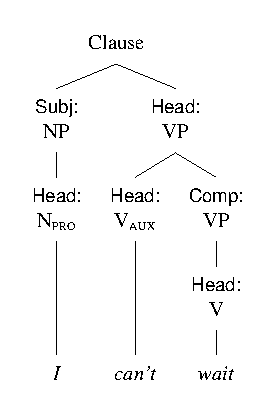
\includegraphics{figures/icantwait.pdf}
    \caption{Syntax trees for \textit{I can't wait} and \textit{I do not ski.}}
    \label{tree:icantwait}

    \centering
    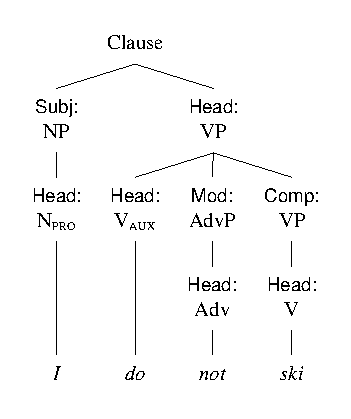
\includegraphics{figures/idonotski.pdf}
%    \label{tree:idonotski}
    \end{multicols}
\end{figure}

This is exactly the same phrase structure as the positive clause \textit{I can wait}, or \textit{she won't fail}, or \textit{you should try}. That's because \textit{can't} is simply the negative form of \textit{can}, \textit{won't} of will, etc.\footnote{In the \textit{CGEL} framework, the complement of the VP is not just a VP but a whole clause, so that \textit{wait} is a verb, which is the head of a VP, which is the head of a clause, and that clause is the complement. This is a better theoretical analysis for reasons I won't go into, but to keep things simple, I'm going to fudge and just call it a VP in this book.} In fact, any clause with a pronoun + auxiliary verb + lexical verb would have this structure.

Similarly, there's nothing at all special about \textit{do} support for negation. A clause like \textit{I do not ski} has exactly the same structure (Figure~\ref{tree:icantwait} again) as \textit{she is always skiing} or \textit{you should really come}.

The only slightly odd structure is negative \is{negation!and imperatives}\textsc{imperatives}, such as \textit{don't worry}, \textit{don't go away}, \textit{don't tell me what to do}, \textit{don't be afraid}, etc. These all require \textit{do} support. Most auxiliary verbs are impossible here, and \textit{be}, while possible, still requires \textit{do} support (Figure~\ref{tree:dontbe}).

\begin{figure}
    \centering
    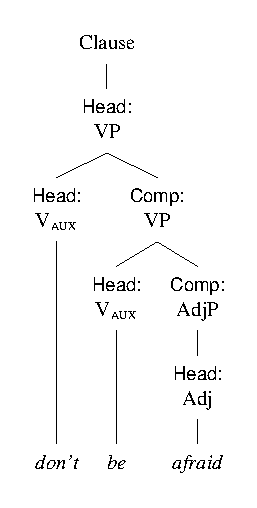
\includegraphics{figures/dontbe.pdf}
    \caption{Syntax tree for \textit{Don't be afraid.}}
    \label{tree:dontbe}
\end{figure}

\subsection{Non-verbal negation}

This is the other kind of clausal negation, but again, there's no special structure. \textit{No} and \textit{neither} are just determiners. The fact that they are negative has no bearing on the phrase structure. The clauses in Figure~\ref{tree:noinjuries} could just as easily be for positive determiners like \textit{some}, \textit{many}, or \textit{all}. Nor would it change for approximate negators like \textit{few}, \textit{a few}, or \textit{hardly any}.

\begin{figure}
    \begin{multicols}{2}
    \centering
    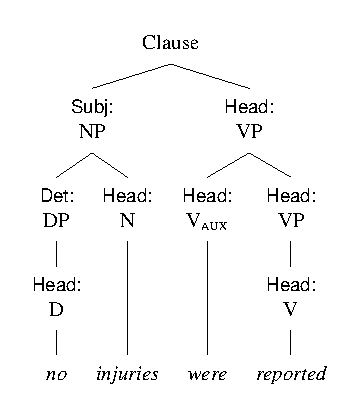
\includegraphics[width=\linewidth]{figures/noinjuries.pdf}
    \caption{Syntax trees for \textit{No injuries were reported} and \textit{Neither side has all the answers.}}
    \label{tree:noinjuries}

    \centering
    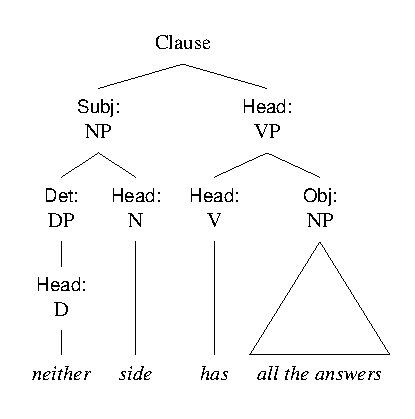
\includegraphics[width=\linewidth]{figures/neitherside.pdf}
    \end{multicols}
\end{figure}

That's not to say there are no interesting constructions at all. There is a slightly older construction~-- COHA suggests its use is fading, while Google Books Ngrams Viewer shows a strong resurgence starting around 2000~-- the \textit{never} + auxiliary verb + subject construction (e.g., \textit{never did he try}. Here \textit{never} has been fronted (like an interrogative phrase, see \ref{sec:subj-aux-inversion-and-fronting}), and this fronting has triggered \is{subject--auxiliary inversion}\is{inversion!subject--auxiliary}subject--auxiliary inversion. As a result, we can expect a structure similar to that in Figure~\ref{fig:what-can-you}. The actual tree structure is shown in Figure~\ref{tree:neverdidhe}\footnote{\textit{Nor did he have any idea}, is a similar example but with a \textsc{coordinator}. See Section \ref{sec:coordination}.}

\begin{figure}
    \centering
    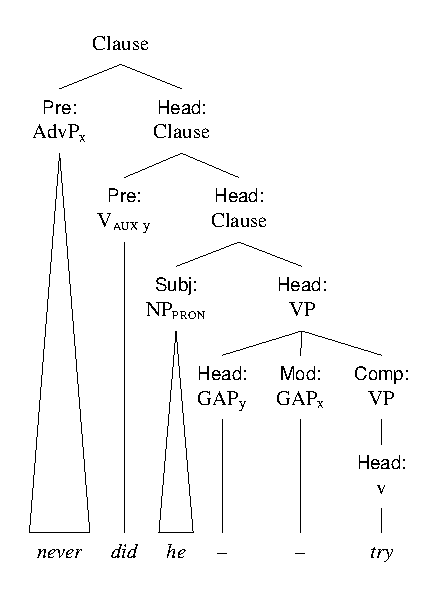
\includegraphics{figures/neverdidhe.pdf}
    \caption{Syntax tree for \textit{Never did he try} with subject--auxiliary inversion.}
    \label{tree:neverdidhe}
\end{figure}

\subsection{Sub-clausal and affixal negation}

I expect you're getting the idea by now that negation poses very few phrase-structure issues. That happy situation continues to hold with sub-clausal negation. Consider the example in Figure~\ref{tree:notforthefirsttime} from (\ref{ex:sub-clausal-negation}). Nothing notable comes of adding the adverb \textit{not}.

\begin{figure}
    \centering
    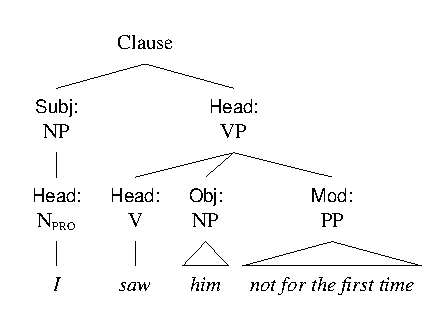
\includegraphics{figures/notforthefirsttime.pdf}
    \caption{Syntax tree for \textit{I saw him not for the first time.}}
    \label{tree:notforthefirsttime}
\end{figure}

And, of course, affixal negation only changes the internal structure of various words; phrase structure is not affected.

\subsection{Summary}

The purpose of the trees, as I've said, is to help you see the syntax at a glance. The trees in this section all recapitulate structures you've seen in previous chapters, providing a good opportunity for review. Deliberate practice (Section \ref{sec:delib}) with drawing trees will be invaluable to you in improving your ability to categorize words and phrases and to understanding phrase structure.
\is{phrase structure|)}
\is{scope|)}
\is{grammaticalization|)}
\is{interrogative clause|)}
\is{contraction|)}
\is{do-support@\textit{do}-support|)}\is{auxiliary do@auxiliary \textit{do}|)}
\is{polarity (positive vs negative)|)}
\is{negation|)}